\chapter{Асуудал ба шийдэл}
Дадлагын хүрээнд "Hoome" платформын микросервисүүд дээр ажиллахад програмчлалын түвшний олон асуудлуудтай тулгарсан бөгөөд шийдлүүдийг хавсаргав.
\section{Админ dashboard}
homebook-metrics сервис нь хэрэглэгчдийн интеракц болон бусад үйл ажиллагаанууд, төлбөр тооцоо бүхий үйл явцыг удирдлагад зориулан харуулах зорилготой бөгөөд  Prometheus, Grafana зэрэг системүүдийг ашигладаг. 

Prometheus-ийг ашиглан тодорхой хугацааны завсар, өдөр тутмын тодорхой цагт өгөгдлийн сангаас уншилт хийж, тухайн уншсан өгөгдлийг HTTP protocol-оор бусад сервисүүдэд нээлттэй болгож өгдөг. Харин Grafana нь тухайн prometheus-ийн scrape хийсэн өгөгдлийг олон граф болон visualize tools ашиглан хэрэглэгчид харуулдаг. 


Эдгээр технологиудыг ашиглан удирдлагын dashboard хийсэн бөгөөд өгөгдлийн сан нь cassandra (CQL) дээр ажилладаг бөгөөд cassandra өгөгдлийн сан нь өгөгдлөө илүү найдвартай ажиллагааны хүрээнд cluster болгон хуваадаг. CQL ашиглан хэрэглэгч бүрийн тохирох датаг уншилт хийхэд өгөгдлийн сангийн зохиомжоос хамааран unique key хийж өгөөгүйгээс үүдэн group-лэх боломжгүй болсон байсан. Үүнээс үүдэн сервис нь бүх датаг өөр дээрээ аван database operation-уудыг хийх болсон билээ. 

Логик: Өгөгдлийн сангаас уншилт хийгээд өөр дээрээ боловсруулан тухайн хэрэгцээт id бүхий хэрэглэгчдийн мэдээллийг keycloak-аас уншиж авах.

Жишээ: \textbf{Хамгийн их like дарсан хэрэглэгчийн тоо}

\begin{lstlisting}[language=Java, frame=single, caption=Materialized view үүсгэн уншилт хийж буй байдал]
SimpleStatement statement = SimpleStatement
  .builder(
      "create materialized view if not exists " +
      keyspaceName +
      ".most_liked_users as select * from reaction where type='UP' and actor is not null and activityid is not null and type is not null and parent is not null and id is not null primary key(actor, activityid, type, parent, id);"
  )
  .setConsistencyLevel(DefaultConsistencyLevel.LOCAL_QUORUM)
  .setTimeout(Duration.ofSeconds(10))
  .build();
session.execute(statement);

PreparedStatement ps = session.prepare("select actor, actorname, count(*) as likes_count from most_liked_users group by actor");
ResultSet rs = session.execute(ps.getQuery());

List<Map.Entry<String, Integer>> list = new ArrayList<>();

for (Row user : rs) {
  list.add(Map.entry(user.getString("actorname"), Math.toIntExact(user.getLong("likes_count"))));
}

return list;
\end{lstlisting}
\pagebreak
\begin{lstlisting}[language=Java, frame=single, caption=Keycloak-аас хэрэглэгчийн мэдээллийг авч буй байдал]
List<Map.Entry<String, Long>> mostLikedUsers = getMostLikedUsers();
mostLikedUsers.sort(Map.Entry.comparingByValue(Comparator.reverseOrder()));

int gaugeBuiltCount = 0;
for (Map.Entry<String, Long> entry : mostLikedUsers) {
    if (gaugeBuiltCount >= mostLikedUsersLimit) {
        break;
    }
    try {
        Gauge
            .builder("homebook.mostLikedUsers", () -> entry.getValue())
            .tag("user_name", getUsernameFromUuid(entry.getKey()))
            .register(registry);
        gaugeBuiltCount++;
    } catch (NotFoundException nfe) {
        log.error("userId: {} not found in keycloak", entry.getKey());
    }
}
return Mono.empty();
\end{lstlisting}

\pagebreak

\section{Retry стратеги}
Kafka image processing consumer сервис нь хэрэглэгчийн оролт буюу оруулсан зурагны хэмжээнээс хамааран compress хийхдээ эхний оролдлогоор exception буцаах асуудлыг илрүүлсэн бөгөөд үүнд Kafka @RetryableTopic annotation-ийг ашигласан хэдий ч тухайн kafka-д зориулсан annotation-ий хөгжүүлэлтийн баригдмал байдлаас үүдэн Spring boot-ийн өөрийн @Retryable болон @Recover annotation-уудыг ашигласан билээ. 

\begin{lstlisting}[language=Java, caption=Retryable-ийг хэрэгжүүлсэн байдал, frame=single]
@KafkaListener(topics = "#{'${kafka.image-topic.topic-name}'}", groupId = "#{'${kafka.image-topic.topic-group-id}'}")
  @Retryable(value = {Exception.class}, maxAttemptsExpression = "#{'${kafka.image-topic.consumer.attempts}'}", backoff = @Backoff(delayExpression = "#{'${kafka.image-topic.consumer.backoff.delay}'}", multiplierExpression = "#{'${kafka.image-topic.consumer.backoff.multiplier}'}"))
  public void consumeMessage(String imageTopicJson) throws Exception {
    // ... Logics
      imageTopic = imageService.process(imageTopic);
      cloudClientService.setObjectStorage(imageTopic);
  }
  @Recover
  public void recoverAfterRetryFail(Exception ex, String imageTopicJson) {
      // ... Logics
      try {
          String exceptionMessage = objectMapper.writeValueAsString(messageMap);
          config.kafkaTemplate().send(dltTopic, exceptionMessage);
      } catch (JsonProcessingException e) {
          e.printStackTrace();
      }
  }
\end{lstlisting}

\begin{figure}[h]
    \centering
    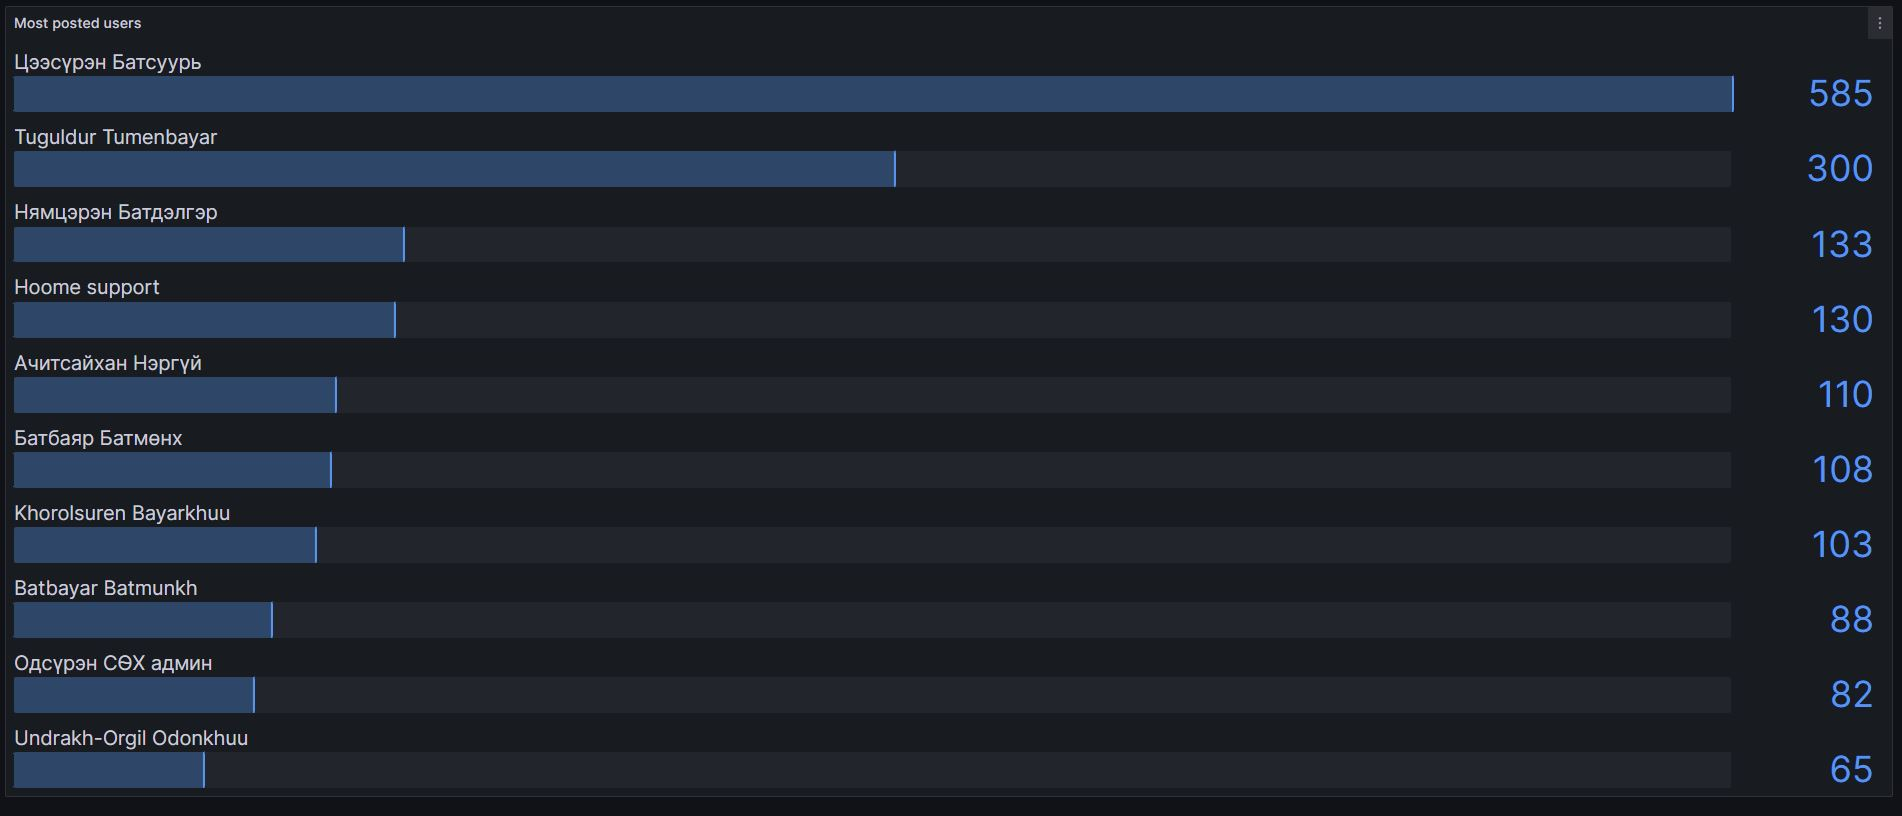
\includegraphics[scale=0.3]{imgs/mostPosted.JPG}
    \caption{Хамгийн их пост хийсэн хэрэглэгчдийн dashboard}
\end{figure}

\begin{figure}[h]
    \centering
    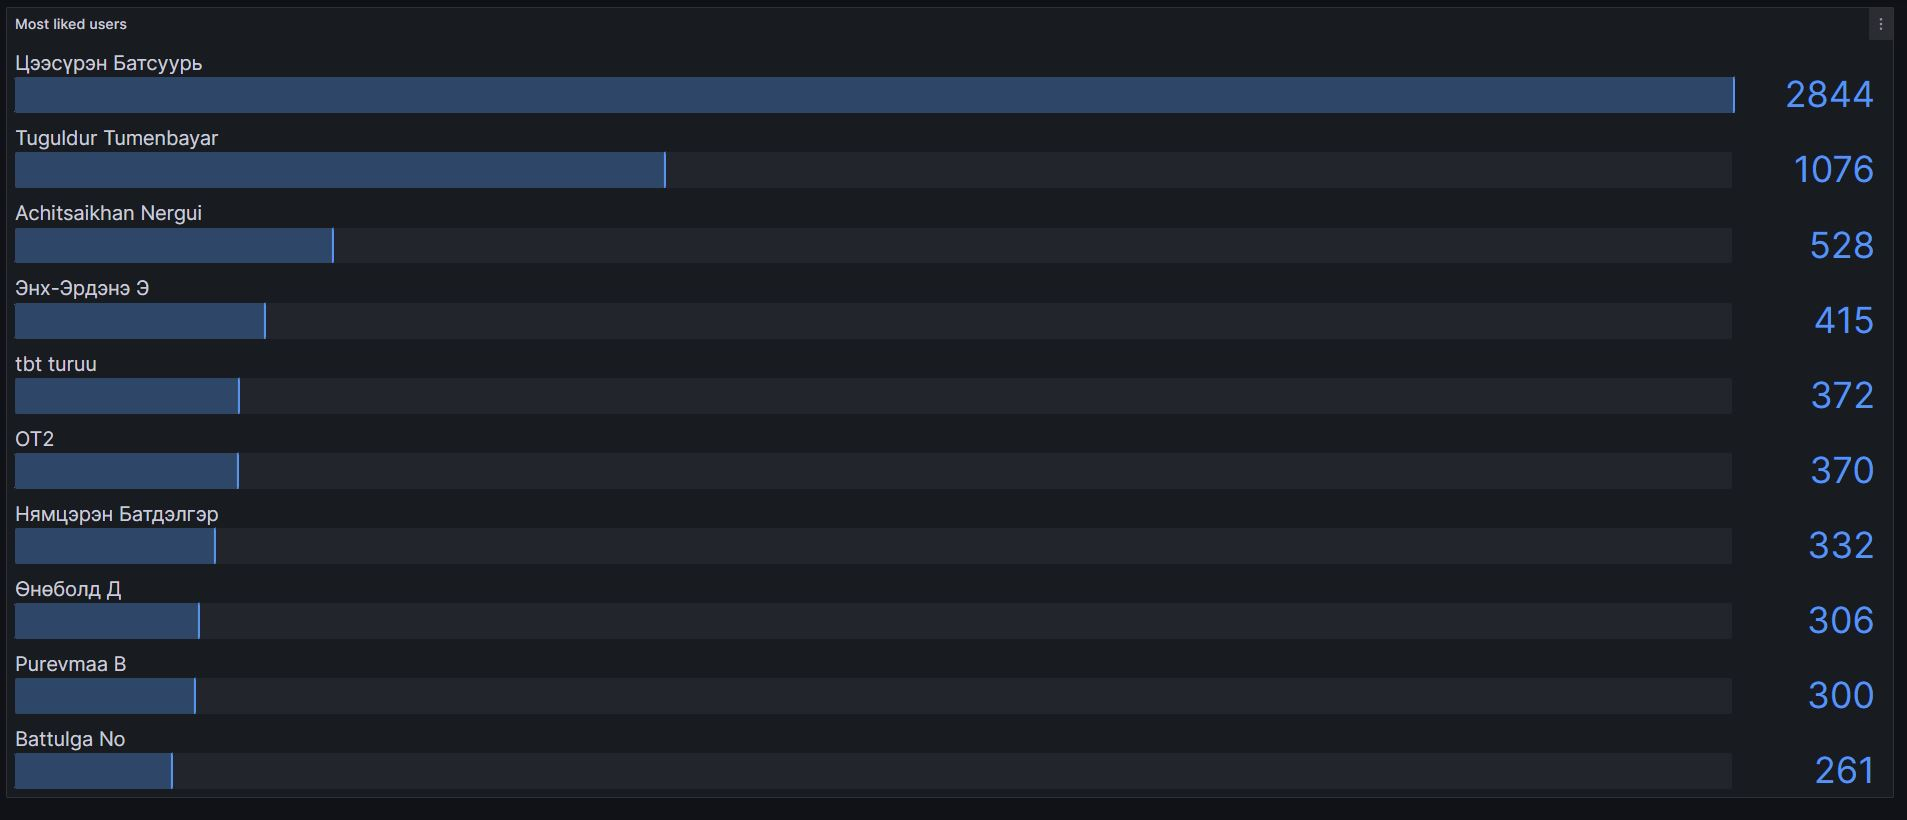
\includegraphics[scale=0.3]{imgs/mostLiked.JPG}
    \caption{Хамгийн их пост хийсэн хэрэглэгчдийн dashboard}
\end{figure}